\documentclass[12pt,a4paper]{report}
\usepackage{vntex} % Tiếng Việt
\usepackage{graphicx} % Chèn hình ảnh
\usepackage{fancyhdr} % Gói hỗ trợ tạo header và footer fancy
\usepackage{changepage} % Thay đổi lề
\usepackage{pdfpages} % Chèn file pdf
% Chèn code
\usepackage{listings} % Thêm gói listings để chèn code
\usepackage{xcolor} % Màu cho code
\lstset{
    language=Matlab,
    basicstyle=\footnotesize\ttfamily,
    numbers=none,
    numberstyle=\tiny\color{gray},
    stepnumber=1,
    numbersep=0.01pt,
    tabsize=2,
    breaklines=true,
    breakatwhitespace=false,
    xleftmargin=0cm, % for line numbers
    framexleftmargin=0cm, % for code frame
    keywordstyle=\color{blue},
    commentstyle=\color{green},
    stringstyle=\color{orange},
    frame=single,
    rulecolor=\color{black},
    basicstyle=\ttfamily,
}

% Footnote, reference and appendix
\usepackage[style=numeric,backend=biber]{biblatex} % Sử dụng gói biblatex
\usepackage{capt-of} %  Footnote trong caption
\usepackage[perpage]{footmisc} % Đánh số lại chú thích mỗi trang
\usepackage[toc,page]{appendix}

% Thiết lập bảng
\usepackage{array} % Gói hỗ trợ các bảng phức tạp
\usepackage{tabularx}
\usepackage{longtable} % Tạo bảng qua nhiều trang
\usepackage{cellspace}
\usepackage{diagbox} % Gói hỗ trợ tạo các ô chéo trong bảng
\usepackage{multirow}
\usepackage{makecell}
\usepackage{adjustbox}

% Thiết lập công thức toán học
\usepackage{amsmath} % Gói hỗ trợ các công thức toán học
\usepackage{amsfonts} % Gói hỗ trợ các ký hiệu toán học
\usepackage{amssymb} % Gói hỗ trợ các ký hiệu toán học
\usepackage{graphicx} % Gói hỗ trợ chèn hình ảnh
\usepackage{bm} % Chữ in đậm trong công thức toán 
\usepackage{physics}

% Thiết lập khác
\usepackage{tikz}
\usepackage{color}
\usepackage{subcaption}
\usepackage{framed}
\usepackage{float} % Để chèn hình ảnh vào đúng vị trí
\usepackage{fancyvrb} % Đưa dữ liệu dạng nguyên thủy vào

% Thiết lập kích thước
\usepackage{geometry}
\geometry{
    left=3cm,
    right=2cm,
    top=2.5cm,
    bottom=2.5cm,
}
\usepackage{hyperref} %Chèn link
\hypersetup{urlcolor=black,linkcolor=black,citecolor=black,colorlinks=true} % Màu cho các đường nét
\everymath{\color{black}}
\setlength{\headheight}{20pt}
\pagestyle{fancy}

%Header
\fancyhead{} % clear all header fields
\fancyhead[L]{
 \begin{tabular}{rl}
    \begin{picture}(25,15)(0,0)
    \put(0,-8){
\includegraphics[width=12mm, height=12mm]{pictures/hcmut.png}}
    %\put(0,-8){\epsfig{width=10mm,figure=hcmut.eps}}
   \end{picture}&
	%
\includegraphics[width=8mm, height=8mm]{hcmut.png} & %
	\begin{tabular}{l}
		\textbf{\bf \ttfamily Trường Đại Học Bách Khoa - ĐHQG TP.Hồ Chí Minh}\\
		\textbf{\bf \ttfamily Khoa Cơ Khí - Bộ môn Cơ điện tử}
	\end{tabular} 	
 \end{tabular}
}
\fancyhead[R]{
	{\tiny \bf \quad} % Khoảng trắng nhỏ trong header bên phải
}

%Footer
\fancyfoot{} % clear all footer fields
\fancyfoot[L]{\scriptsize \ttfamily Động lực học và điều khiển}
\fancyfoot[R]{\scriptsize \ttfamily Trang {\thepage}/9}
\renewcommand{\headrulewidth}{0.3pt}
\renewcommand{\footrulewidth}{0.3pt}
\renewcommand{\thesection}{\arabic{section}}
\begin{document}
    \begin{titlepage}   
    \begin{center}
        \vspace*{-2cm} 
        \large
        \textbf{ĐẠI HỌC QUỐC GIA THÀNH PHỐ HỒ CHÍ MINH \\
        TRƯỜNG ĐẠI HỌC BÁCH KHOA\\
        KHOA CƠ KHÍ\\
        BỘ MÔN CƠ ĐIỆN TỬ}\\
        
\includegraphics[width=70mm, height=70mm]{pictures/hcmut.png} \\
        \rule{\linewidth}{0.5mm}\\
        \vspace{0.8cm}
        \Large
        \textbf{BÁO CÁO BÀI TẬP LỚN \\VI ĐIỀU KHIỂN}\\
        \vspace*{0.5cm}
        \Huge
        \textbf{ĐIỀU KHIỂN ĐÈN GIAO THÔNG}\\
        \vspace{0.5cm}
        \rule{\linewidth}{0.5mm}\\
        \vspace{0.8cm}
        \vspace{1cm}
        \large
        \textbf{GVHD: TS. PHÙNG THANH HUY}\\
        \vspace{0.5cm}
        SINH VIÊN THỰC HIỆN:\\[0.3cm]
        \begin{tabular}{|>{\centering\arraybackslash}m{5cm}|>{\centering\arraybackslash}m{7cm}|>{\centering\arraybackslash}m{5cm}|}
            \hline
            \textbf{Họ và tên} & \textbf{MSSV} \\
            \hline
            Đào Trọng Chân & 2210350 \\
            \hline
            Trần Quang Đạo & 2210647 \\
            \hline
            Võ Hữu Dư & 2210604 \\
            \hline
            Dương Quang Duy & 2210497 \\
            \hline
        \end{tabular}
    \end{center}
        
    \vfill
    \large
    \begin{center}
        TP.HCM, \today
    \end{center}
\end{titlepage}

    \section*{LỜI CẢM ƠN}

Trước tiên, nhóm sinh viên chúng em xin được bày tỏ lòng biết ơn chân thành và sâu sắc đến TS. Phùng Thanh Huy, người đã trực tiếp giảng dạy và hướng dẫn nhóm trong suốt quá trình thực hiện bài tập lớn môn Vi điều khiển. Thầy không chỉ truyền đạt cho chúng em những kiến thức chuyên môn vững chắc, mà còn định hướng tư duy kỹ thuật và phương pháp làm việc khoa học, cẩn trọng – những hành trang vô cùng quý báu cho chúng em trong quá trình học tập và nghiên cứu sau này.

Trong suốt quá trình triển khai đề tài “Hệ thống điều khiển đèn giao thông sử dụng vi điều khiển PIC16F887”, chúng em đã có cơ hội tiếp cận với nhiều kỹ thuật lập trình nhúng, thiết kế mạch nguyên lý, mô phỏng hệ thống thực tế bằng Proteus, cũng như quản lý tiến độ và phối hợp nhóm hiệu quả. Đây là một trải nghiệm vừa thử thách vừa bổ ích, giúp chúng em rèn luyện kỹ năng tư duy logic, giải quyết vấn đề và làm việc nhóm trong môi trường kỹ thuật.

Chúng em cũng xin gửi lời cảm ơn chân thành đến quý thầy cô trong Bộ môn Cơ điện tử – Khoa Cơ khí – Trường Đại học Bách Khoa – Đại học Quốc gia TP.HCM, những người đã không ngừng cống hiến cho công tác giảng dạy, tạo dựng môi trường học tập hiện đại, năng động, giúp sinh viên phát triển toàn diện về năng lực chuyên môn và phẩm chất nghề nghiệp.

Chúng em xin chân thành cảm ơn!

\vspace{0.5cm}
\hfill TP. Hồ Chí Minh, ngày 01 tháng 05 năm 2025

    \tableofcontents
    \cleardoublepage 
    \section{Nguyên lý hoạt động}
\subsection{Chuyển chế độ}
\begin{figure}[H]
    \centering
    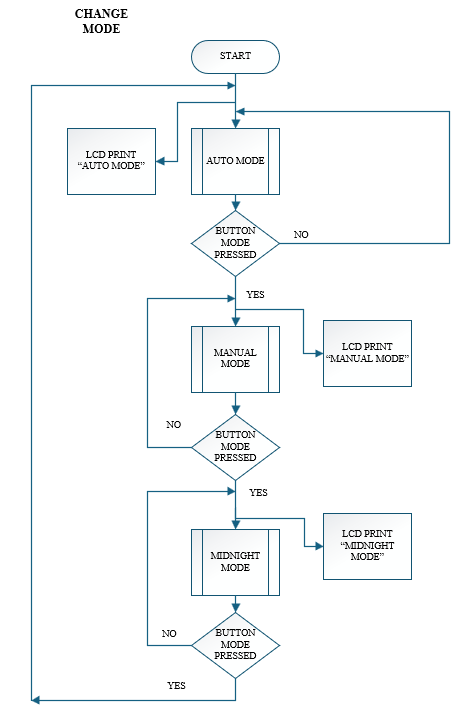
\includegraphics[width=0.8\textwidth]{pictures/modes.png}
    \caption{Lưu đồ chuyển chế độ}
\end{figure}
\cleardoublepage
Lưu đồ chuyển chế độ mô tả trình tự xử lý nút nhấn để thay đổi chế độ hoạt động của hệ thống đèn giao thông. Sau khi khởi động, hệ thống bắt đầu ở chế độ AUTO MODE, đồng thời hiển thị dòng chữ “AUTO MODE” trên LCD. Trong mỗi chế độ, hệ thống liên tục kiểm tra xem nút MODE có được nhấn hay không:
\begin{itemize}
    \item Chế độ mặc định là chế độ tự động (AUTO MODE).
    \item Nếu nút nhấn chuyển trạng thái không được nhấn, hệ thống tiếp tục duy trì chế độ hiện tại.
    \item Nếu nút nhấn chuyển trạng thái được nhấn, hệ thống sẽ chuyển sang chế độ tiếp theo trong danh sách chế độ hoạt động. 
    \item Sau mỗi lần chuyển chế độ LCD sẽ cập nhật lại dòng chữ hiển thị chế độ tương ứng.
\end{itemize}
\subsection{Chế độ tự động}
\begin{figure}[H]
    \centering
    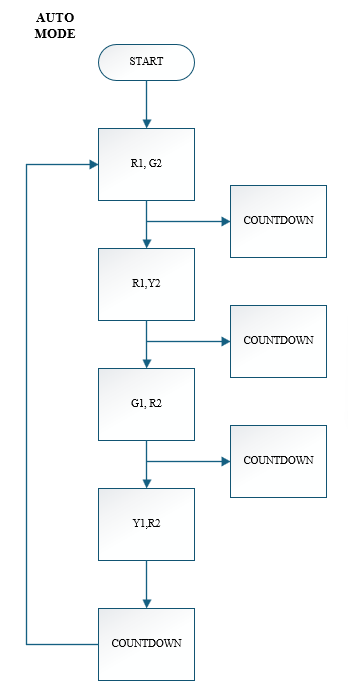
\includegraphics[width=0.45\textwidth]{pictures/auto.png}
    \caption{Lưu đồ chế độ tự động}
\end{figure}
\cleardoublepage
Chế độ tự động mô phỏng hoạt động thực tế của hệ thống đèn giao thông. Lưu đồ mô tả thứ tự bật/tắt đèn theo chu kỳ, kết hợp với bộ đếm thời gian:
\begin{enumerate}
    \item Bật \textbf{R1, G2} $\rightarrow$ đếm ngược
    \item Bật \textbf{R1, Y2} $\rightarrow$ đếm ngược
    \item Bật \textbf{G1, R2} $\rightarrow$ đếm ngược
    \item Bật \textbf{Y1, R2} $\rightarrow$ đếm ngược
\end{enumerate}


Sau bước cuối, hệ thống quay lại bước đầu tiên để lặp lại chu kỳ. Đây là chế độ giao thông tiêu chuẩn cho hai hướng đối diện.
\subsection{Chế độ thủ công}
\begin{figure}[H]
    \centering
    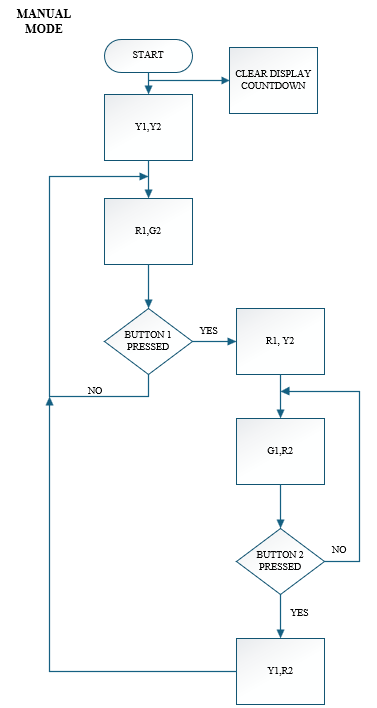
\includegraphics[width=0.7\textwidth]{pictures/manual.png}
    \caption{Lưu đồ chế độ thủ công}
\end{figure}
\cleardoublepage
Trong chế độ này, người dùng chủ động điều khiển các giai đoạn đèn giao thông thông qua nút nhấn.

Trình tự hoạt động như sau:

\begin{enumerate}
  \item Bật \textbf{R1, G2}
  \item Chờ nhấn \textbf{BUTTON 1}. Nếu không nhấn, giữ nguyên trạng thái.
  \item Nếu BUTTON 1 được nhấn, chuyển sang \textbf{G1, R2}
  \item Chờ nhấn \textbf{BUTTON 2}. Nếu không nhấn, giữ nguyên trạng thái.
  \item Nếu BUTTON 2 được nhấn, chuyển sang \textbf{R1, G2}, sau đó quay lại bước đầu tiên.
\end{enumerate}

Chế độ này thích hợp để điều phối giao thông theo yêu cầu trong các tình huống đặc biệt.

\subsection{Chế độ ban đêm}
\begin{figure}[H]
    \centering
    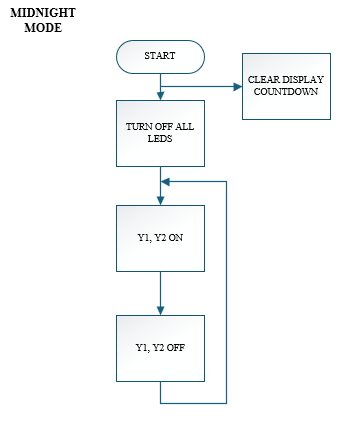
\includegraphics[width=0.7\textwidth]{pictures/night.png}
    \caption{Lưu đồ chế độ ban đêm}
\end{figure}
\cleardoublepage
Chế độ ban đêm giúp tiết kiệm điện năng và tăng cảnh báo cho các phương tiện giao thông khi lưu lượng thấp. Trình tự hoạt động:

\begin{enumerate}
  \item Khởi động và xóa màn hình LCD
  \item Tắt toàn bộ đèn (\textbf{OFF ALL LEDs})
  \item Bật \textbf{Y1, Y2} $\rightarrow$ đèn vàng hai hướng sáng
  \item Tắt \textbf{Y1, Y2}
  \item Quay lại bước bật Y1, Y2 để tạo hiệu ứng nhấp nháy liên tục
\end{enumerate}

Chế độ này đảm bảo cảnh báo tối thiểu nhưng không gây cản trở phương tiện trong đêm khuya.
    \section{Mô phỏng với proteus}
Để kiểm tra và đánh giá hoạt động của hệ thống điều khiển đèn giao thông, nhóm đã sử dụng phần mềm \textbf{Proteus} để mô phỏng toàn bộ mạch điện và chương trình điều khiển. Mô phỏng giúp phát hiện các lỗi logic, kiểm tra chính xác thứ tự hoạt động của các đèn và đảm bảo hệ thống vận hành đúng như thiết kế trước khi triển khai thực tế. \\

Mục tiêu mô phỏng:
\begin{itemize}
    \item Xác thực logic điều khiển trong từng chế độ hoạt động.
    \item Đảm bảo đèn giao thông chuyển pha đúng thứ tự và đúng thời gian.
    \item Kiểm tra hiển thị trên LCD và LED 7 đoạn có hoạt động chính xác hay không.
    \item Kiểm tra tín hiệu từ các nút nhấn có được vi điều khiển nhận đúng không.
\end{itemize}
\subsection{Mô phỏng chế độ tự động}
\begin{figure}[H]
    \centering
    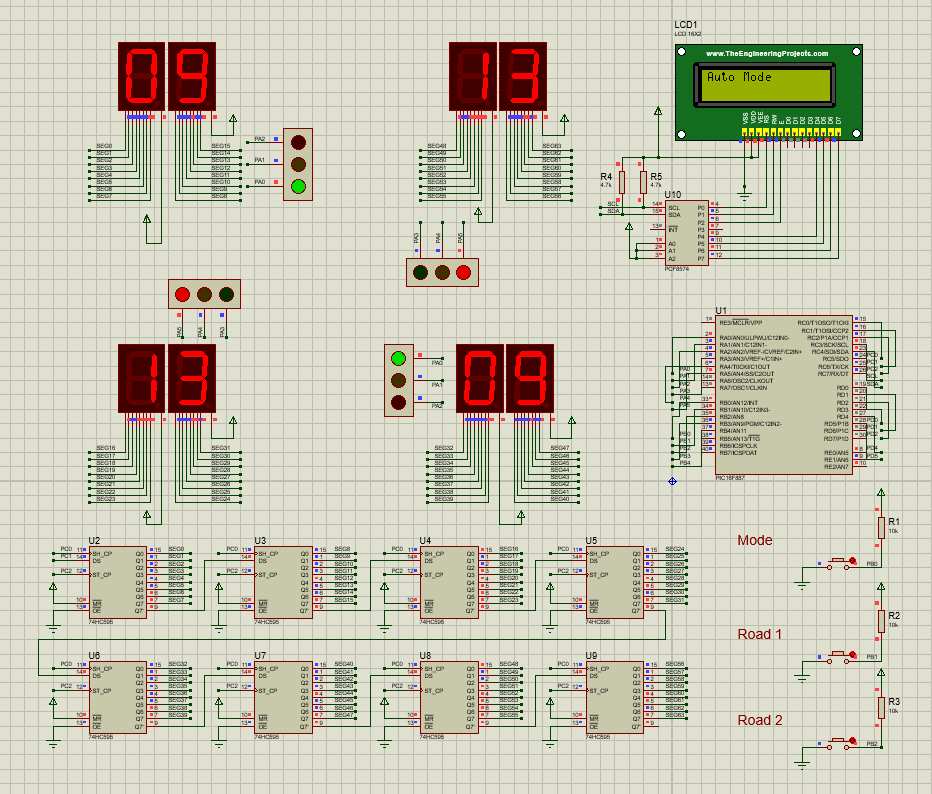
\includegraphics[width=0.7\textwidth]{pictures/autoproteus.png}
    \caption{Mô phỏng chế độ tự động với Proteus}
\end{figure}
Khi bắt đầu mô phỏng, hệ thống khởi động ở chế độ mặc định là \textbf{AUTO MODE}. LCD hiển thị dòng chữ “AUTO MODE”. Các cụm đèn giao thông hoạt động tuần tự theo 4 pha chính:
\begin{enumerate}
    \item Đèn đỏ hướng 1 (R1) sáng, đèn xanh hướng 2 (G2) sáng, đếm ngược.
    \item Đèn đỏ hướng 1 (R1) sáng, đèn vàng hướng 2 (Y2) sáng, đếm ngược.
    \item Đèn xanh hướng 1 (G1) sáng, đèn đỏ hướng 2 (R2) sáng, đếm ngược.
    \item Đèn vàng hướng 1 (Y1) sáng, đèn đỏ hướng 2 (R2) sáng, đếm ngược.
\end{enumerate}
Các LED 7 đoạn hiển thị thời gian đếm ngược tương ứng với từng pha.

\subsection{Mô phỏng chế độ thủ công}
\begin{figure}[H]
    \centering
    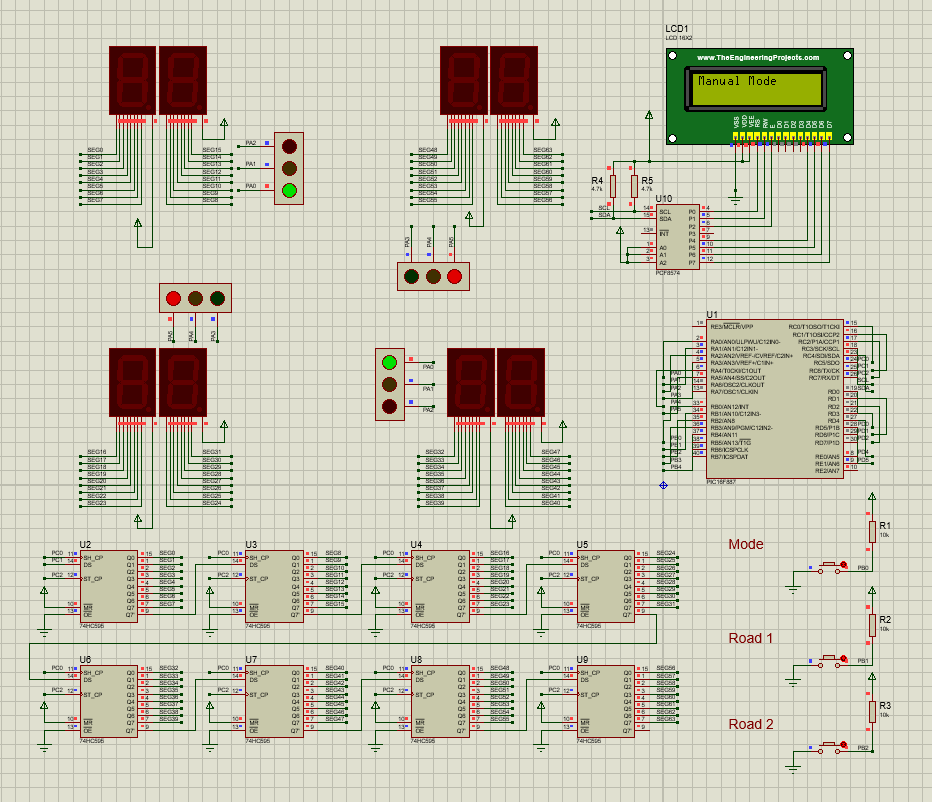
\includegraphics[width=0.7\textwidth]{pictures/manualproteus.png}
    \caption{Mô phỏng chế độ thủ công với Proteus}
\end{figure}
Khi nhấn nút MODE, hệ thống chuyển sang \textbf{MANUAL MODE}, LCD cập nhật dòng chữ tương ứng. Ở chế độ này:
\begin{itemize}
    \item Người dùng nhấn \texttt{BUTTON1} để chuyển từ pha R1-G2 sang G1-R2.
    \item Nhấn \texttt{BUTTON2} để chuyển từ G1-R2 sang Y1-R2.
    \item Sau đó hệ thống quay lại pha đầu tiên.
\end{itemize}
Trong mô phỏng, trạng thái đèn chỉ thay đổi khi có thao tác từ người dùng, giúp kiểm soát giao thông linh hoạt trong tình huống đặc biệt.


\subsection{Mô phỏng chế độ ban đêm}
\begin{figure}[H]
    \centering
    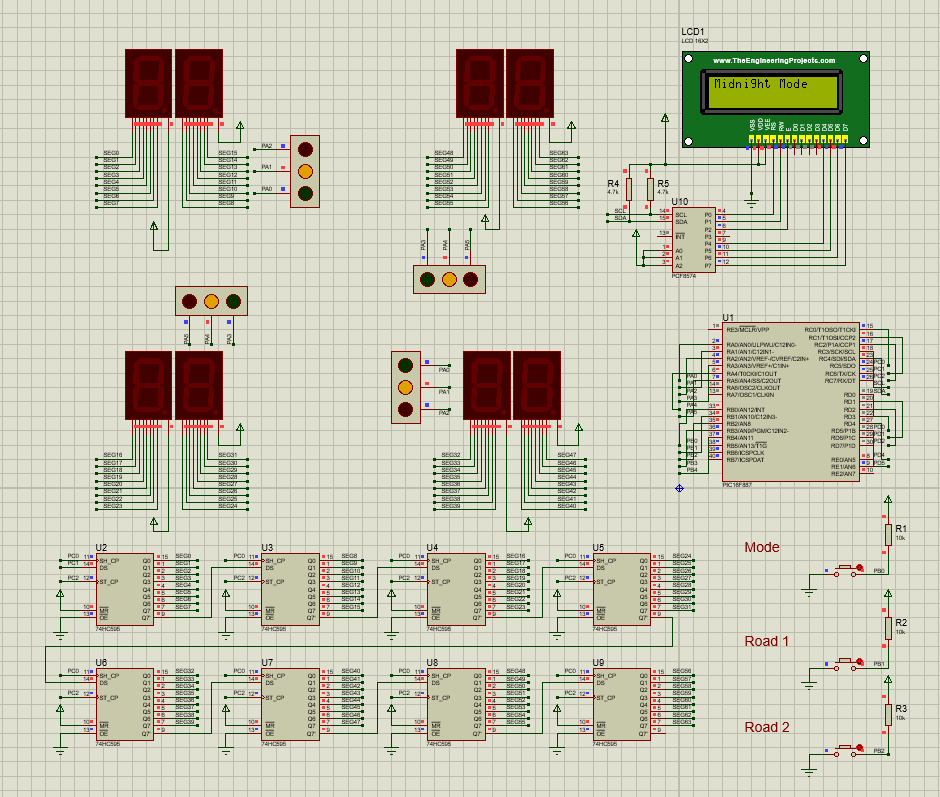
\includegraphics[width=0.7\textwidth]{pictures/nightproteus.png}
    \caption{Mô phỏng chế độ ban đêm với Proteus}
\end{figure}
Khi nhấn MODE lần nữa, hệ thống chuyển sang \textbf{NIGHT MODE}. LCD hiển thị “NIGHT MODE”. Tất cả đèn giao thông sẽ tắt, chỉ còn đèn vàng (Y1, Y2) của hai hướng nhấp nháy liên tục để cảnh báo. Điều này được thể hiện rõ trong mô phỏng bằng hiệu ứng bật/tắt liên tục với chu kỳ đều đặn.
\subsection{Nhận xét và đánh giá}
\begin{itemize}
    \item Các chế độ hoạt động đúng như thiết kế và chương trình đã lập trình.
    \item Đèn giao thông chuyển pha chính xác, không có tình trạng xung đột tín hiệu.
    \item LCD và LED 7 đoạn hoạt động ổn định, hiển thị đúng nội dung.
    \item Việc sử dụng Proteus giúp nhóm tiết kiệm thời gian thử nghiệm phần cứng, đồng thời kiểm tra logic chương trình một cách trực quan và hiệu quả.
\end{itemize}
$\Rightarrow$ Tiến hành xây dựng phần cứng thực tế.
\cleardoublepage
    \section{Các linh kiện chính}
\renewcommand{\arraystretch}{1.5} % Tăng khoảng cách giữa các dòng
\begin{center}
\begin{tabular}{|c|c|c|>{\centering\arraybackslash}m{3cm}|}
    \hline
    \textbf{STT} & \textbf{Tên linh kiện} & \textbf{Số lượng} & \textbf{Hình ảnh} \\
    \hline
    1 & PIC16F887 & 1 & 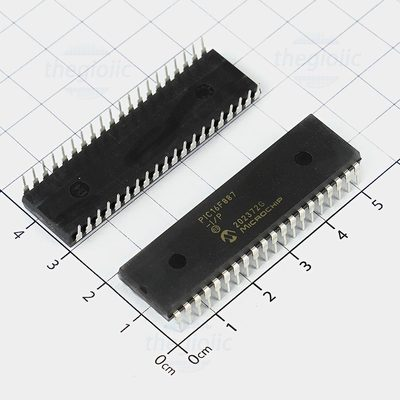
\includegraphics[width=2.5cm]{pictures/pic16f887.png} \\
    \hline
    2 & Đế ra chân PIC & 1 & 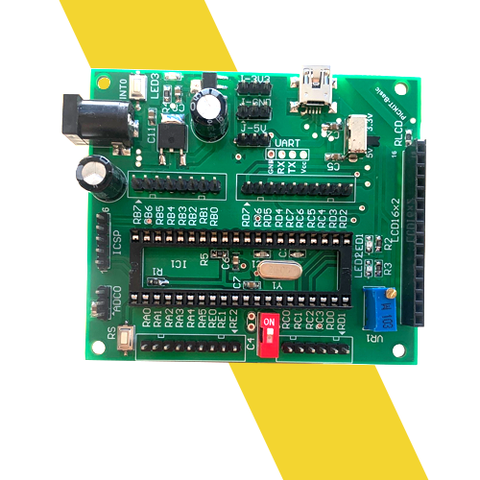
\includegraphics[width=2.5cm]{pictures/kitpic.png} \\
    \hline
    3 & Mạch đèn giao thông & 4 & 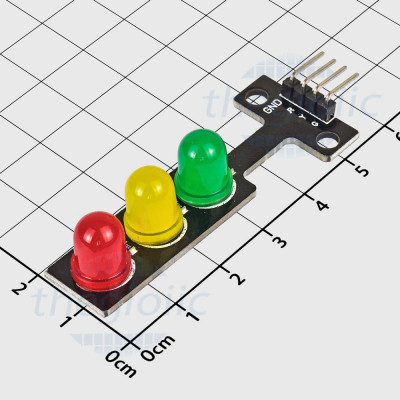
\includegraphics[width=2.5cm]{pictures/traficlight.png} \\
    \hline
    4 & Module 2 LED 7 đoạn 74HC595  & 4 & 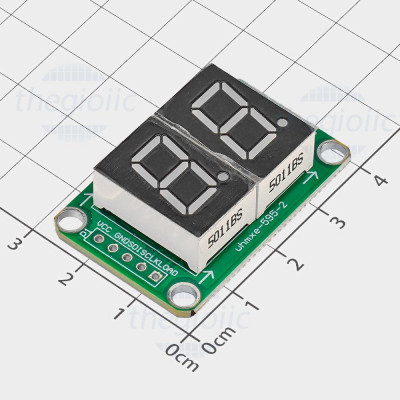
\includegraphics[width=2.5cm]{pictures/7led.png} \\
    \hline
    5 & LCD 1602 & 1 & 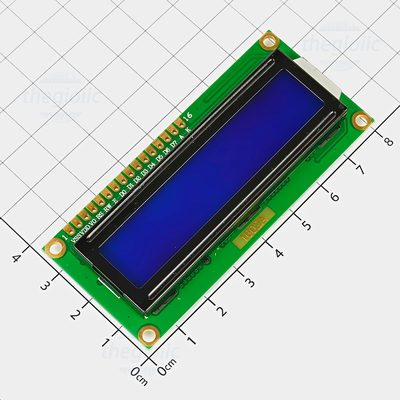
\includegraphics[width=2.5cm]{pictures/lcd.png} \\
    \hline
    6 & Mạch giao tiếp LCD I2C & 1 & 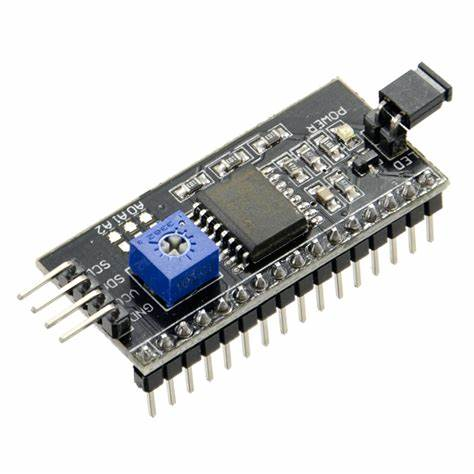
\includegraphics[width=2.5cm]{pictures/i2c.png} \\
    \hline
    7 & Nút nhấn & 3 & 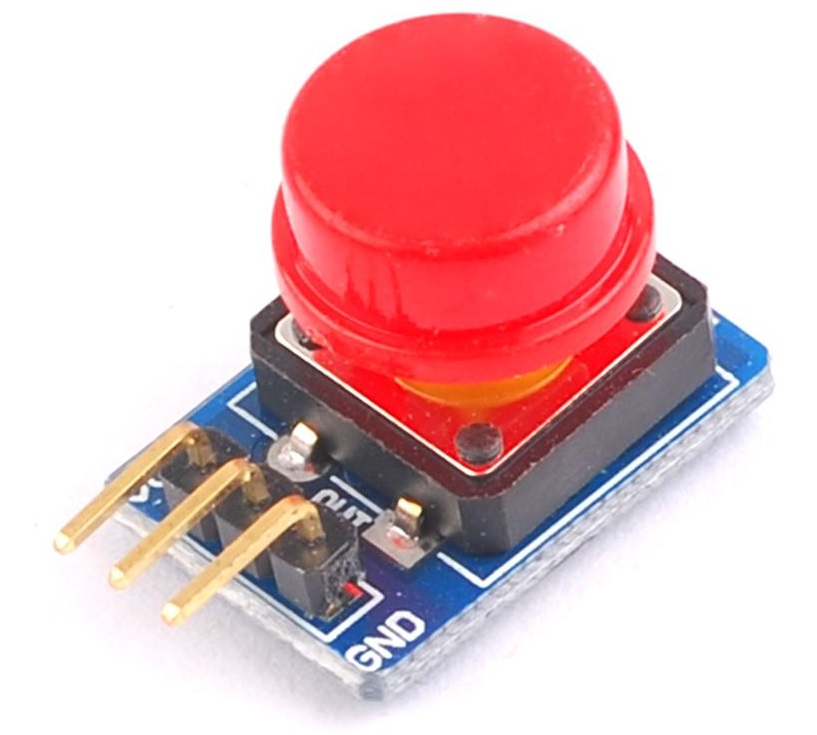
\includegraphics[width=2.5cm]{pictures/button.png} \\
    \hline
\end{tabular}
\end{center}
\cleardoublepage
\textbf{Mô tả chức năng các linh kiện chính}
\begin{itemize}
    \item \textbf{PIC16F887}: Vi điều khiển chính điều khiển toàn bộ hoạt động của hệ thống, bao gồm xử lý chế độ, điều khiển đèn, hiển thị và đọc nút nhấn.
    \item \textbf{Đế ra chân PIC}: Dùng để cố định và kết nối PIC16F887 với breadboard hoặc mạch in, thuận tiện cho lắp ráp và tháo rời.
    \item \textbf{Mạch đèn giao thông}: Gồm 3 LED (đỏ, vàng, xanh) mô phỏng các tín hiệu giao thông ở ngã tư.
    \item \textbf{Module 2 LED 7 đoạn 74HC595}: Hiển thị thời gian đếm ngược trong từng pha đèn, được điều khiển thông qua IC dịch 74HC595 nhằm giảm số lượng chân I/O của vi điều khiển.
    \item \textbf{LCD 1602}: Hiển thị chế độ hoạt động của hệ thống (AUTO, MANUAL, NIGHT), giúp người dùng dễ dàng theo dõi trạng thái.
    \item \textbf{Module I2C giao tiếp LCD}: Cho phép kết nối LCD với vi điều khiển qua giao tiếp I2C, giảm số lượng chân cần dùng.
    \item \textbf{Nút nhấn}: Dùng để chuyển đổi chế độ hoạt động và điều khiển pha đèn trong chế độ thủ công.
\end{itemize}
\cleardoublepage
    \section{Sơ đồ nguyên lý}
\subsection{Vi điều khiển PIC16F887}
\begin{figure}[H]
    \centering
    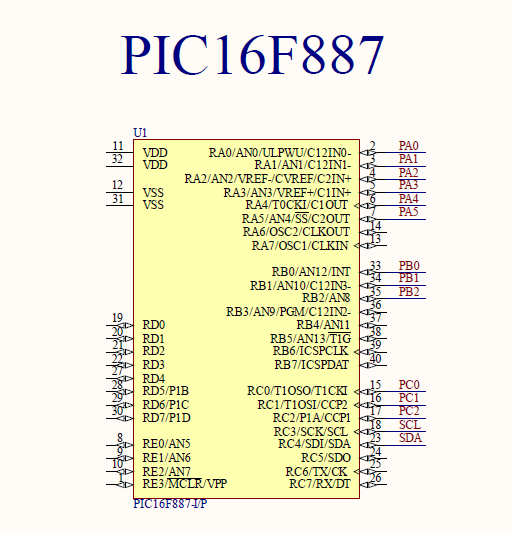
\includegraphics[width=0.7\textwidth]{pictures/pic_sch.png}
\end{figure}
Là trung tâm xử lý điều khiển toàn bộ hệ thống. Các chân I/O của vi điều khiển được cấu hình để:
\begin{itemize}
    \item Giao tiếp với LED qua IC dịch 74HC595.
    \item Đọc trạng thái nút nhấn để chuyển chế độ.
    \item Giao tiếp LCD qua giao tiếp I2C (sử dụng module PCF8574).
\end{itemize}
Các chân của vi điều khiển được sử dụng trong mạch như sau:
\begin{itemize}
    \item \texttt{RA0 -- RA5}: Điều khiển các cụm đèn LED giao thông (đỏ, vàng, xanh) cho từng hướng.
    \item \texttt{RB0 -- RB2}: Nhận tín hiệu từ 3 nút nhấn dùng để chuyển chế độ hoạt động và chuyển pha đèn trong chế độ thủ công.
    \item \texttt{RC3 (SCL)} và \texttt{RC4 (SDA)}: Giao tiếp I2C với module PCF8574T để điều khiển LCD 1602.
    \item \texttt{RC0 -- RC2}: Giao tiếp với IC 74HC595 để đồng bộ hóa dữ liệu xuất ra LED 7 đoạn.
\end{itemize}

\subsection{IC dịch 74HC595 và mạch hiển thị 7 đoạn}
\begin{figure}[H]
    \centering
    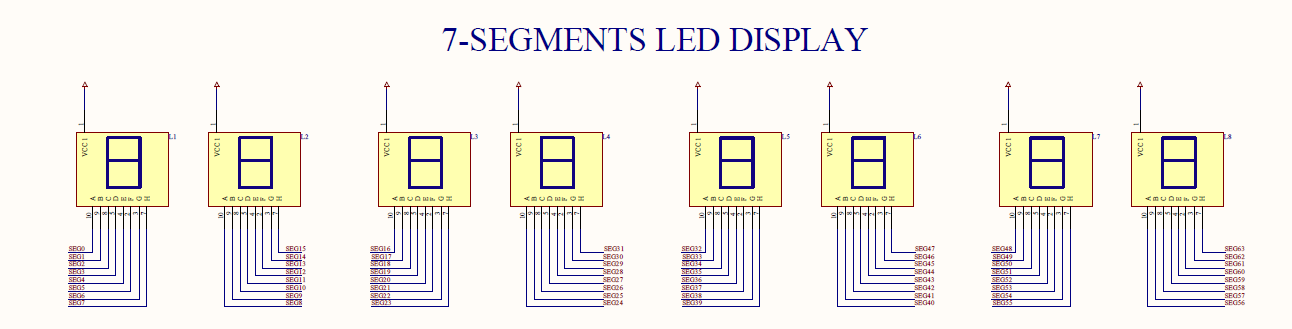
\includegraphics[width=1\textwidth]{pictures/7seg1.png}
\end{figure}
\begin{figure}[H]
    \centering
    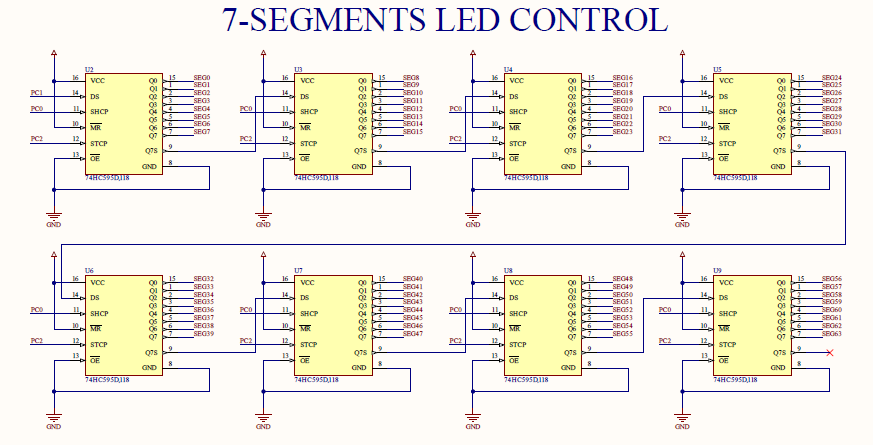
\includegraphics[width=1\textwidth]{pictures/7seg2.png}
\end{figure}
Để tiết kiệm chân I/O của vi điều khiển, hệ thống sử dụng 8 IC 74HC595 để điều khiển nhiều LED 7 đoạn hiển thị đếm ngược thời gian cho các pha đèn. Mỗi IC điều khiển một cụm 8 LED. Cách hoạt động như sau:
\begin{itemize}
    \item Dữ liệu nhị phân từ PIC được dịch nối tiếp qua các IC 74HC595.
    \item Các chân \texttt{SHCP}, \texttt{STCP} và \texttt{DS} được điều khiển nhịp nhàng để đẩy dữ liệu ra song song.
    \item Tín hiệu hiển thị số được mã hóa theo bảng BCD và cập nhật liên tục theo từng pha đèn.
\end{itemize}

\subsection{LCD 1602 giao tiếp I2C}
\begin{figure}[H]
    \centering
    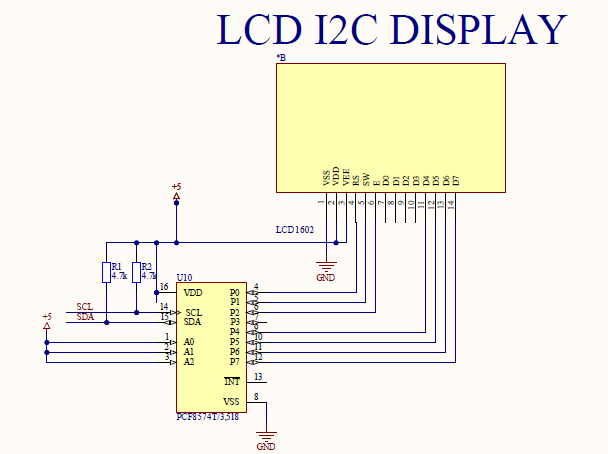
\includegraphics[width=0.7\textwidth]{pictures/lcd_sch.png}
\end{figure}

Màn hình LCD dùng để hiển thị chế độ hiện tại của hệ thống: AUTO MODE, MANUAL MODE, hay NIGHT MODE. Module I2C giao tiếp LCD cho phép điều khiển LCD chỉ với 2 dây:
\begin{itemize}
    \item \texttt{SDA (RC4)}: Truyền dữ liệu.
    \item \texttt{SCL (RC3)}: Truyền xung clock.
\end{itemize}
Sử dụng mô dun giao tiếp LCD I2C giúp giảm số lượng chân cần sử dụng, từ 6--8 chân xuống còn 2, rất hữu ích cho các hệ thống có số lượng chân giới hạn.

    \section{Mô hình hệ thống hoàn chỉnh}

\cleardoublepage
    \section{Kết luận}

Sau quá trình tìm hiểu, thiết kế và thực hiện, nhóm đã hoàn thành đề tài “Hệ thống điều khiển đèn giao thông sử dụng vi điều khiển PIC16F887”. Hệ thống đã được lập trình đầy đủ các chức năng, bao gồm ba chế độ hoạt động: \textit{tự động}, \textit{thủ công}, và \textit{ban đêm}. Thông qua việc mô phỏng trên phần mềm Proteus, nhóm đã kiểm tra được tính đúng đắn của thuật toán điều khiển cũng như hoạt động phối hợp của các phần tử trong hệ thống.

Thông qua đề tài, nhóm đã củng cố và nâng cao các kiến thức về:
\begin{itemize}
    \item Lập trình vi điều khiển PIC bằng ngôn ngữ C.
    \item Thiết kế mạch nguyên lý và mạch điều khiển sử dụng LED, LCD, IC dịch 74HC595.
    \item Kỹ năng mô phỏng hệ thống điện tử với Proteus.
    \item Tư duy xử lý tín hiệu, thời gian và chế độ hoạt động trong hệ thống điều khiển thực tế.
\end{itemize}

Bên cạnh những kết quả đạt được, nhóm cũng nhận ra một số điểm cần cải thiện, chẳng hạn như tối ưu hóa mã nguồn, nâng cao tính thẩm mỹ khi mô phỏng, và tăng cường tính thực tế nếu triển khai hệ thống ngoài thực tế (ví dụ: sử dụng cảm biến phát hiện phương tiện, tích hợp RTC, hoặc giao tiếp không dây).

Qua bài tập lớn này, nhóm không chỉ có thêm kiến thức thực tiễn trong lĩnh vực vi điều khiển mà còn rèn luyện được kỹ năng làm việc nhóm, tư duy phân tích hệ thống và cách thức xây dựng một dự án kỹ thuật từ khâu thiết kế đến kiểm thử. Đây là tiền đề quan trọng cho các môn học, đồ án chuyên ngành và công việc kỹ sư sau này.
\cleardoublepage

\end{document}